\documentclass[twoside]{book}

% Packages required by doxygen
\usepackage{fixltx2e}
\usepackage{calc}
\usepackage{doxygen}
\usepackage[export]{adjustbox} % also loads graphicx
\usepackage{graphicx}
\usepackage[utf8]{inputenc}
\usepackage{makeidx}
\usepackage{multicol}
\usepackage{multirow}
\PassOptionsToPackage{warn}{textcomp}
\usepackage{textcomp}
\usepackage[nointegrals]{wasysym}
\usepackage[table]{xcolor}

% Font selection
\usepackage[T1]{fontenc}
\usepackage[scaled=.90]{helvet}
\usepackage{courier}
\usepackage{amssymb}
\usepackage{sectsty}
\renewcommand{\familydefault}{\sfdefault}
\allsectionsfont{%
  \fontseries{bc}\selectfont%
  \color{darkgray}%
}
\renewcommand{\DoxyLabelFont}{%
  \fontseries{bc}\selectfont%
  \color{darkgray}%
}
\newcommand{\+}{\discretionary{\mbox{\scriptsize$\hookleftarrow$}}{}{}}

% Page & text layout
\usepackage{geometry}
\geometry{%
  a4paper,%
  top=2.5cm,%
  bottom=2.5cm,%
  left=2.5cm,%
  right=2.5cm%
}
\tolerance=750
\hfuzz=15pt
\hbadness=750
\setlength{\emergencystretch}{15pt}
\setlength{\parindent}{0cm}
\setlength{\parskip}{3ex plus 2ex minus 2ex}
\makeatletter
\renewcommand{\paragraph}{%
  \@startsection{paragraph}{4}{0ex}{-1.0ex}{1.0ex}{%
    \normalfont\normalsize\bfseries\SS@parafont%
  }%
}
\renewcommand{\subparagraph}{%
  \@startsection{subparagraph}{5}{0ex}{-1.0ex}{1.0ex}{%
    \normalfont\normalsize\bfseries\SS@subparafont%
  }%
}
\makeatother

% Headers & footers
\usepackage{fancyhdr}
\pagestyle{fancyplain}
\fancyhead[LE]{\fancyplain{}{\bfseries\thepage}}
\fancyhead[CE]{\fancyplain{}{}}
\fancyhead[RE]{\fancyplain{}{\bfseries\leftmark}}
\fancyhead[LO]{\fancyplain{}{\bfseries\rightmark}}
\fancyhead[CO]{\fancyplain{}{}}
\fancyhead[RO]{\fancyplain{}{\bfseries\thepage}}
\fancyfoot[LE]{\fancyplain{}{}}
\fancyfoot[CE]{\fancyplain{}{}}
\fancyfoot[RE]{\fancyplain{}{\bfseries\scriptsize Generated by Doxygen }}
\fancyfoot[LO]{\fancyplain{}{\bfseries\scriptsize Generated by Doxygen }}
\fancyfoot[CO]{\fancyplain{}{}}
\fancyfoot[RO]{\fancyplain{}{}}
\renewcommand{\footrulewidth}{0.4pt}
\renewcommand{\chaptermark}[1]{%
  \markboth{#1}{}%
}
\renewcommand{\sectionmark}[1]{%
  \markright{\thesection\ #1}%
}

% Indices & bibliography
\usepackage{natbib}
\usepackage[titles]{tocloft}
\setcounter{tocdepth}{3}
\setcounter{secnumdepth}{5}
\makeindex

% Hyperlinks (required, but should be loaded last)
\usepackage{ifpdf}
\ifpdf
  \usepackage[pdftex,pagebackref=true]{hyperref}
\else
  \usepackage[ps2pdf,pagebackref=true]{hyperref}
\fi
\hypersetup{%
  colorlinks=true,%
  linkcolor=blue,%
  citecolor=blue,%
  unicode%
}

% Custom commands
\newcommand{\clearemptydoublepage}{%
  \newpage{\pagestyle{empty}\cleardoublepage}%
}

\usepackage{caption}
\captionsetup{labelsep=space,justification=centering,font={bf},singlelinecheck=off,skip=4pt,position=top}

%===== C O N T E N T S =====

\begin{document}

% Titlepage & ToC
\hypersetup{pageanchor=false,
             bookmarksnumbered=true,
             pdfencoding=unicode
            }
\pagenumbering{alph}
\begin{titlepage}
\vspace*{7cm}
\begin{center}%
{\Large Elevator Simulator \\[1ex]\large 1.\+0.\+0.\+1 }\\
\vspace*{1cm}
{\large Generated by Doxygen 1.8.13}\\
\end{center}
\end{titlepage}
\clearemptydoublepage
\pagenumbering{roman}
\tableofcontents
\clearemptydoublepage
\pagenumbering{arabic}
\hypersetup{pageanchor=true}

%--- Begin generated contents ---
\chapter{Namespace Index}
\section{Packages}
Here are the packages with brief descriptions (if available)\+:\begin{DoxyCompactList}
\item\contentsline{section}{\hyperlink{namespacecn}{cn} }{\pageref{namespacecn}}{}
\item\contentsline{section}{\hyperlink{namespacecn_1_1leonwong}{cn.\+leonwong} }{\pageref{namespacecn_1_1leonwong}}{}
\item\contentsline{section}{\hyperlink{namespacecn_1_1leonwong_1_1_elevator_simulator}{cn.\+leonwong.\+Elevator\+Simulator} }{\pageref{namespacecn_1_1leonwong_1_1_elevator_simulator}}{}
\item\contentsline{section}{\hyperlink{namespacecn_1_1leonwong_1_1_elevator_simulator_1_1_model}{cn.\+leonwong.\+Elevator\+Simulator.\+Model} }{\pageref{namespacecn_1_1leonwong_1_1_elevator_simulator_1_1_model}}{}
\end{DoxyCompactList}

\chapter{Hierarchical Index}
\section{Class Hierarchy}
This inheritance list is sorted roughly, but not completely, alphabetically\+:\begin{DoxyCompactList}
\item \contentsline{section}{cn.\+leonwong.\+Elevator\+Simulator.\+Model.\+Building}{\pageref{classcn_1_1leonwong_1_1_elevator_simulator_1_1_model_1_1_building}}{}
\item \contentsline{section}{cn.\+leonwong.\+Elevator\+Simulator.\+Model.\+Message}{\pageref{classcn_1_1leonwong_1_1_elevator_simulator_1_1_model_1_1_message}}{}
\item \contentsline{section}{cn.\+leonwong.\+Elevator\+Simulator.\+Model.\+Passenger}{\pageref{classcn_1_1leonwong_1_1_elevator_simulator_1_1_model_1_1_passenger}}{}
\item Thread\begin{DoxyCompactList}
\item \contentsline{section}{cn.\+leonwong.\+Elevator\+Simulator.\+Controller}{\pageref{classcn_1_1leonwong_1_1_elevator_simulator_1_1_controller}}{}
\item \contentsline{section}{cn.\+leonwong.\+Elevator\+Simulator.\+Model.\+Elevator}{\pageref{classcn_1_1leonwong_1_1_elevator_simulator_1_1_model_1_1_elevator}}{}
\end{DoxyCompactList}
\item Application\begin{DoxyCompactList}
\item \contentsline{section}{cn.\+leonwong.\+Elevator\+Simulator.\+View}{\pageref{classcn_1_1leonwong_1_1_elevator_simulator_1_1_view}}{}
\end{DoxyCompactList}
\end{DoxyCompactList}

\chapter{Class Index}
\section{Class List}
Here are the classes, structs, unions and interfaces with brief descriptions\+:\begin{DoxyCompactList}
\item\contentsline{section}{\hyperlink{classcn_1_1leonwong_1_1_elevator_simulator_1_1_model_1_1_building}{cn.\+leonwong.\+Elevator\+Simulator.\+Model.\+Building} }{\pageref{classcn_1_1leonwong_1_1_elevator_simulator_1_1_model_1_1_building}}{}
\item\contentsline{section}{\hyperlink{classcn_1_1leonwong_1_1_elevator_simulator_1_1_controller}{cn.\+leonwong.\+Elevator\+Simulator.\+Controller} }{\pageref{classcn_1_1leonwong_1_1_elevator_simulator_1_1_controller}}{}
\item\contentsline{section}{\hyperlink{classcn_1_1leonwong_1_1_elevator_simulator_1_1_model_1_1_elevator}{cn.\+leonwong.\+Elevator\+Simulator.\+Model.\+Elevator} }{\pageref{classcn_1_1leonwong_1_1_elevator_simulator_1_1_model_1_1_elevator}}{}
\item\contentsline{section}{\hyperlink{classcn_1_1leonwong_1_1_elevator_simulator_1_1_model_1_1_message}{cn.\+leonwong.\+Elevator\+Simulator.\+Model.\+Message} }{\pageref{classcn_1_1leonwong_1_1_elevator_simulator_1_1_model_1_1_message}}{}
\item\contentsline{section}{\hyperlink{classcn_1_1leonwong_1_1_elevator_simulator_1_1_model_1_1_passenger}{cn.\+leonwong.\+Elevator\+Simulator.\+Model.\+Passenger} }{\pageref{classcn_1_1leonwong_1_1_elevator_simulator_1_1_model_1_1_passenger}}{}
\item\contentsline{section}{\hyperlink{classcn_1_1leonwong_1_1_elevator_simulator_1_1_view}{cn.\+leonwong.\+Elevator\+Simulator.\+View} }{\pageref{classcn_1_1leonwong_1_1_elevator_simulator_1_1_view}}{}
\end{DoxyCompactList}

\chapter{File Index}
\section{File List}
Here is a list of all files with brief descriptions\+:\begin{DoxyCompactList}
\item\contentsline{section}{src/cn/leonwong/\+Elevator\+Simulator/\hyperlink{_controller_8java}{Controller.\+java} }{\pageref{_controller_8java}}{}
\item\contentsline{section}{src/cn/leonwong/\+Elevator\+Simulator/\hyperlink{_view_8java}{View.\+java} }{\pageref{_view_8java}}{}
\item\contentsline{section}{src/cn/leonwong/\+Elevator\+Simulator/\+Model/\hyperlink{_building_8java}{Building.\+java} }{\pageref{_building_8java}}{}
\item\contentsline{section}{src/cn/leonwong/\+Elevator\+Simulator/\+Model/\hyperlink{_elevator_8java}{Elevator.\+java} }{\pageref{_elevator_8java}}{}
\item\contentsline{section}{src/cn/leonwong/\+Elevator\+Simulator/\+Model/\hyperlink{_message_8java}{Message.\+java} }{\pageref{_message_8java}}{}
\item\contentsline{section}{src/cn/leonwong/\+Elevator\+Simulator/\+Model/\hyperlink{_passenger_8java}{Passenger.\+java} }{\pageref{_passenger_8java}}{}
\end{DoxyCompactList}

\chapter{Namespace Documentation}
\hypertarget{namespacecn}{}\section{Package cn}
\label{namespacecn}\index{cn@{cn}}
\subsection*{Packages}
\begin{DoxyCompactItemize}
\item 
package \hyperlink{namespacecn_1_1leonwong}{leonwong}
\end{DoxyCompactItemize}

\hypertarget{namespacecn_1_1leonwong}{}\section{Package cn.\+leonwong}
\label{namespacecn_1_1leonwong}\index{cn.\+leonwong@{cn.\+leonwong}}
\subsection*{Packages}
\begin{DoxyCompactItemize}
\item 
package \hyperlink{namespacecn_1_1leonwong_1_1_elevator_simulator}{Elevator\+Simulator}
\end{DoxyCompactItemize}

\hypertarget{namespacecn_1_1leonwong_1_1_elevator_simulator}{}\section{Package cn.\+leonwong.\+Elevator\+Simulator}
\label{namespacecn_1_1leonwong_1_1_elevator_simulator}\index{cn.\+leonwong.\+Elevator\+Simulator@{cn.\+leonwong.\+Elevator\+Simulator}}
\subsection*{Packages}
\begin{DoxyCompactItemize}
\item 
package \hyperlink{namespacecn_1_1leonwong_1_1_elevator_simulator_1_1_model}{Model}
\end{DoxyCompactItemize}
\subsection*{Classes}
\begin{DoxyCompactItemize}
\item 
class \hyperlink{classcn_1_1leonwong_1_1_elevator_simulator_1_1_controller}{Controller}
\item 
class \hyperlink{classcn_1_1leonwong_1_1_elevator_simulator_1_1_view}{View}
\end{DoxyCompactItemize}

\hypertarget{namespacecn_1_1leonwong_1_1_elevator_simulator_1_1_model}{}\section{Package cn.\+leonwong.\+Elevator\+Simulator.\+Model}
\label{namespacecn_1_1leonwong_1_1_elevator_simulator_1_1_model}\index{cn.\+leonwong.\+Elevator\+Simulator.\+Model@{cn.\+leonwong.\+Elevator\+Simulator.\+Model}}
\subsection*{Classes}
\begin{DoxyCompactItemize}
\item 
class \hyperlink{classcn_1_1leonwong_1_1_elevator_simulator_1_1_model_1_1_building}{Building}
\item 
class \hyperlink{classcn_1_1leonwong_1_1_elevator_simulator_1_1_model_1_1_elevator}{Elevator}
\item 
class \hyperlink{classcn_1_1leonwong_1_1_elevator_simulator_1_1_model_1_1_message}{Message}
\item 
class \hyperlink{classcn_1_1leonwong_1_1_elevator_simulator_1_1_model_1_1_passenger}{Passenger}
\end{DoxyCompactItemize}

\chapter{Class Documentation}
\hypertarget{classcn_1_1leonwong_1_1_elevator_simulator_1_1_model_1_1_building}{}\section{cn.\+leonwong.\+Elevator\+Simulator.\+Model.\+Building Class Reference}
\label{classcn_1_1leonwong_1_1_elevator_simulator_1_1_model_1_1_building}\index{cn.\+leonwong.\+Elevator\+Simulator.\+Model.\+Building@{cn.\+leonwong.\+Elevator\+Simulator.\+Model.\+Building}}
\subsection*{Public Member Functions}
\begin{DoxyCompactItemize}
\item 
\hyperlink{classcn_1_1leonwong_1_1_elevator_simulator_1_1_model_1_1_building_a1e083b2c0741e1b45d620401f67b51c3}{Building} (int levs, int elevs, int max\+Pass)
\item 
int \hyperlink{classcn_1_1leonwong_1_1_elevator_simulator_1_1_model_1_1_building_a3cadfe7c0bcba1c58da3e4813985d713}{get\+Elevators} ()
\item 
int \hyperlink{classcn_1_1leonwong_1_1_elevator_simulator_1_1_model_1_1_building_a140ef7ab3469607bd537c51b3da5b833}{get\+Levels} ()
\end{DoxyCompactItemize}
\subsection*{Public Attributes}
\begin{DoxyCompactItemize}
\item 
\mbox{\Hypertarget{classcn_1_1leonwong_1_1_elevator_simulator_1_1_model_1_1_building_a8317933aa9a1de07f64a8de984e19551}\label{classcn_1_1leonwong_1_1_elevator_simulator_1_1_model_1_1_building_a8317933aa9a1de07f64a8de984e19551}} 
Vector$<$ \hyperlink{classcn_1_1leonwong_1_1_elevator_simulator_1_1_model_1_1_elevator}{Elevator} $>$ \hyperlink{classcn_1_1leonwong_1_1_elevator_simulator_1_1_model_1_1_building_a8317933aa9a1de07f64a8de984e19551}{elevator\+List}
\begin{DoxyCompactList}\small\item\em Note for each elevator in this building. \end{DoxyCompactList}\item 
\mbox{\Hypertarget{classcn_1_1leonwong_1_1_elevator_simulator_1_1_model_1_1_building_ae720233ad2086c6f427facb19df4fb33}\label{classcn_1_1leonwong_1_1_elevator_simulator_1_1_model_1_1_building_ae720233ad2086c6f427facb19df4fb33}} 
Vector$<$ Vector$<$ \hyperlink{classcn_1_1leonwong_1_1_elevator_simulator_1_1_model_1_1_passenger}{Passenger} $>$ $>$ \hyperlink{classcn_1_1leonwong_1_1_elevator_simulator_1_1_model_1_1_building_ae720233ad2086c6f427facb19df4fb33}{level\+List}
\begin{DoxyCompactList}\small\item\em Note for persons waiting for elevators in each level. \end{DoxyCompactList}\item 
\mbox{\Hypertarget{classcn_1_1leonwong_1_1_elevator_simulator_1_1_model_1_1_building_a01f6bba8a7c8f2a26a34f7ee8c055275}\label{classcn_1_1leonwong_1_1_elevator_simulator_1_1_model_1_1_building_a01f6bba8a7c8f2a26a34f7ee8c055275}} 
Vector$<$ \hyperlink{classcn_1_1leonwong_1_1_elevator_simulator_1_1_model_1_1_message}{Message} $>$ \hyperlink{classcn_1_1leonwong_1_1_elevator_simulator_1_1_model_1_1_building_a01f6bba8a7c8f2a26a34f7ee8c055275}{message\+Center}
\begin{DoxyCompactList}\small\item\em A message center noting for events;. \end{DoxyCompactList}\end{DoxyCompactItemize}


\subsection{Detailed Description}
\hyperlink{classcn_1_1leonwong_1_1_elevator_simulator_1_1_model_1_1_building}{Building} Simulator Creates a building with given levels and elevators 

\subsection{Constructor \& Destructor Documentation}
\mbox{\Hypertarget{classcn_1_1leonwong_1_1_elevator_simulator_1_1_model_1_1_building_a1e083b2c0741e1b45d620401f67b51c3}\label{classcn_1_1leonwong_1_1_elevator_simulator_1_1_model_1_1_building_a1e083b2c0741e1b45d620401f67b51c3}} 
\index{cn\+::leonwong\+::\+Elevator\+Simulator\+::\+Model\+::\+Building@{cn\+::leonwong\+::\+Elevator\+Simulator\+::\+Model\+::\+Building}!Building@{Building}}
\index{Building@{Building}!cn\+::leonwong\+::\+Elevator\+Simulator\+::\+Model\+::\+Building@{cn\+::leonwong\+::\+Elevator\+Simulator\+::\+Model\+::\+Building}}
\subsubsection{\texorpdfstring{Building()}{Building()}}
{\footnotesize\ttfamily cn.\+leonwong.\+Elevator\+Simulator.\+Model.\+Building.\+Building (\begin{DoxyParamCaption}\item[{int}]{levs,  }\item[{int}]{elevs,  }\item[{int}]{max\+Pass }\end{DoxyParamCaption})}

Creates a building 
\begin{DoxyParams}{Parameters}
{\em levs} & \#levels in ths building \\
\hline
{\em elevs} & \#elevators in this building \\
\hline
{\em max\+Pass} & max \# of passengers an elevator can contain \\
\hline
\end{DoxyParams}


\subsection{Member Function Documentation}
\mbox{\Hypertarget{classcn_1_1leonwong_1_1_elevator_simulator_1_1_model_1_1_building_a3cadfe7c0bcba1c58da3e4813985d713}\label{classcn_1_1leonwong_1_1_elevator_simulator_1_1_model_1_1_building_a3cadfe7c0bcba1c58da3e4813985d713}} 
\index{cn\+::leonwong\+::\+Elevator\+Simulator\+::\+Model\+::\+Building@{cn\+::leonwong\+::\+Elevator\+Simulator\+::\+Model\+::\+Building}!get\+Elevators@{get\+Elevators}}
\index{get\+Elevators@{get\+Elevators}!cn\+::leonwong\+::\+Elevator\+Simulator\+::\+Model\+::\+Building@{cn\+::leonwong\+::\+Elevator\+Simulator\+::\+Model\+::\+Building}}
\subsubsection{\texorpdfstring{get\+Elevators()}{getElevators()}}
{\footnotesize\ttfamily int cn.\+leonwong.\+Elevator\+Simulator.\+Model.\+Building.\+get\+Elevators (\begin{DoxyParamCaption}{ }\end{DoxyParamCaption})}

getter for numbers of elevators \begin{DoxyReturn}{Returns}
numbers of elevators in this building 
\end{DoxyReturn}
\mbox{\Hypertarget{classcn_1_1leonwong_1_1_elevator_simulator_1_1_model_1_1_building_a140ef7ab3469607bd537c51b3da5b833}\label{classcn_1_1leonwong_1_1_elevator_simulator_1_1_model_1_1_building_a140ef7ab3469607bd537c51b3da5b833}} 
\index{cn\+::leonwong\+::\+Elevator\+Simulator\+::\+Model\+::\+Building@{cn\+::leonwong\+::\+Elevator\+Simulator\+::\+Model\+::\+Building}!get\+Levels@{get\+Levels}}
\index{get\+Levels@{get\+Levels}!cn\+::leonwong\+::\+Elevator\+Simulator\+::\+Model\+::\+Building@{cn\+::leonwong\+::\+Elevator\+Simulator\+::\+Model\+::\+Building}}
\subsubsection{\texorpdfstring{get\+Levels()}{getLevels()}}
{\footnotesize\ttfamily int cn.\+leonwong.\+Elevator\+Simulator.\+Model.\+Building.\+get\+Levels (\begin{DoxyParamCaption}{ }\end{DoxyParamCaption})}

getter for numbers of levels \begin{DoxyReturn}{Returns}
numbers of levels in this building 
\end{DoxyReturn}


The documentation for this class was generated from the following file\+:\begin{DoxyCompactItemize}
\item 
src/cn/leonwong/\+Elevator\+Simulator/\+Model/Building.\+java\end{DoxyCompactItemize}

\hypertarget{classcn_1_1leonwong_1_1_elevator_simulator_1_1_controller}{}\section{cn.\+leonwong.\+Elevator\+Simulator.\+Controller Class Reference}
\label{classcn_1_1leonwong_1_1_elevator_simulator_1_1_controller}\index{cn.\+leonwong.\+Elevator\+Simulator.\+Controller@{cn.\+leonwong.\+Elevator\+Simulator.\+Controller}}


Inheritance diagram for cn.\+leonwong.\+Elevator\+Simulator.\+Controller\+:

\hypertarget{classcn_1_1leonwong_1_1_elevator_simulator_1_1_model_1_1_elevator}{}\section{cn.\+leonwong.\+Elevator\+Simulator.\+Model.\+Elevator Class Reference}
\label{classcn_1_1leonwong_1_1_elevator_simulator_1_1_model_1_1_elevator}\index{cn.\+leonwong.\+Elevator\+Simulator.\+Model.\+Elevator@{cn.\+leonwong.\+Elevator\+Simulator.\+Model.\+Elevator}}
Inheritance diagram for cn.\+leonwong.\+Elevator\+Simulator.\+Model.\+Elevator\+:\begin{figure}[H]
\begin{center}
\leavevmode
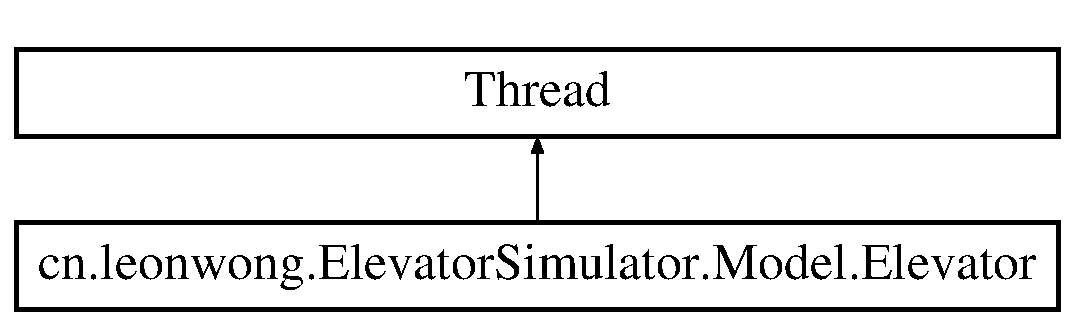
\includegraphics[height=2.000000cm]{classcn_1_1leonwong_1_1_elevator_simulator_1_1_model_1_1_elevator}
\end{center}
\end{figure}
\subsection*{Classes}
\begin{DoxyCompactItemize}
\item 
class {\bfseries Direction}
\end{DoxyCompactItemize}
\subsection*{Public Member Functions}
\begin{DoxyCompactItemize}
\item 
void \hyperlink{classcn_1_1leonwong_1_1_elevator_simulator_1_1_model_1_1_elevator_a45bf0b0add86d6c9f4624aa91804d3c9}{start} ()
\item 
void \hyperlink{classcn_1_1leonwong_1_1_elevator_simulator_1_1_model_1_1_elevator_af9cb9d7e34873bc531ec71aa4ed3deae}{run} ()
\item 
\mbox{\Hypertarget{classcn_1_1leonwong_1_1_elevator_simulator_1_1_model_1_1_elevator_a40f92b8d5f76462a4894e4b4bd670458}\label{classcn_1_1leonwong_1_1_elevator_simulator_1_1_model_1_1_elevator_a40f92b8d5f76462a4894e4b4bd670458}} 
String {\bfseries to\+String} ()
\item 
\hyperlink{classcn_1_1leonwong_1_1_elevator_simulator_1_1_model_1_1_elevator_a8cdebccdd3505647fe57df5ea4315c1a}{Elevator} (int name, int max, int max\+Pass, Vector$<$ Vector$<$ \hyperlink{classcn_1_1leonwong_1_1_elevator_simulator_1_1_model_1_1_passenger}{Passenger} $>$ $>$ levs, Vector$<$ \hyperlink{classcn_1_1leonwong_1_1_elevator_simulator_1_1_model_1_1_message}{Message} $>$ mess, Reentrant\+Lock l)
\item 
boolean \hyperlink{classcn_1_1leonwong_1_1_elevator_simulator_1_1_model_1_1_elevator_a6abc5ffe66c8be2d11493fb9d9a2022f}{is\+Full} ()
\item 
boolean \hyperlink{classcn_1_1leonwong_1_1_elevator_simulator_1_1_model_1_1_elevator_a524eaa48c98d600d587c9e81f47e477b}{is\+Empty} ()
\item 
boolean \hyperlink{classcn_1_1leonwong_1_1_elevator_simulator_1_1_model_1_1_elevator_afef928208c5445a18af5d567ce9a4467}{is\+Idle} ()
\item 
void \hyperlink{classcn_1_1leonwong_1_1_elevator_simulator_1_1_model_1_1_elevator_ad735b8fd22b1b990a02caa95a9c8b96f}{add\+Destination} (int dest)
\item 
int \hyperlink{classcn_1_1leonwong_1_1_elevator_simulator_1_1_model_1_1_elevator_a393eaa2daf4a00730685de6efb3893d5}{get\+Level} ()
\item 
int \hyperlink{classcn_1_1leonwong_1_1_elevator_simulator_1_1_model_1_1_elevator_a0a386b72bfc7edf9a64dcc342dd27f51}{get\+Direction} ()
\item 
int \hyperlink{classcn_1_1leonwong_1_1_elevator_simulator_1_1_model_1_1_elevator_acc5b1cdd5cefc853a1cd33e6e986b3a0}{get\+Max\+Destination} ()
\item 
int \hyperlink{classcn_1_1leonwong_1_1_elevator_simulator_1_1_model_1_1_elevator_a9aeca7de346d6a46aea0692a60e57681}{get\+Min\+Destination} ()
\item 
int \hyperlink{classcn_1_1leonwong_1_1_elevator_simulator_1_1_model_1_1_elevator_acd5f3b902008c64175d9b5c035e8d77f}{get\+Passengers} ()
\item 
void \hyperlink{classcn_1_1leonwong_1_1_elevator_simulator_1_1_model_1_1_elevator_aadee7a0c9b8e13427d46a9f907dcee94}{set\+Level} (int l)
\item 
void \hyperlink{classcn_1_1leonwong_1_1_elevator_simulator_1_1_model_1_1_elevator_a838e6a91c1e6d1ed2786efc462c48151}{stop\+Thread} ()
\item 
String \hyperlink{classcn_1_1leonwong_1_1_elevator_simulator_1_1_model_1_1_elevator_aca1fa93441f3463aece03f01591efa61}{get\+Destinations} ()
\item 
int \hyperlink{classcn_1_1leonwong_1_1_elevator_simulator_1_1_model_1_1_elevator_a8e71679aa5ed47ac62be7d4193f81055}{get\+Destination\+Size} ()
\end{DoxyCompactItemize}
\subsection*{Static Public Attributes}
\begin{DoxyCompactItemize}
\item 
\mbox{\Hypertarget{classcn_1_1leonwong_1_1_elevator_simulator_1_1_model_1_1_elevator_af9cc2a12533172485e7539f3690b2af9}\label{classcn_1_1leonwong_1_1_elevator_simulator_1_1_model_1_1_elevator_af9cc2a12533172485e7539f3690b2af9}} 
static final int \hyperlink{classcn_1_1leonwong_1_1_elevator_simulator_1_1_model_1_1_elevator_af9cc2a12533172485e7539f3690b2af9}{F\+L\+O\+O\+R\+\_\+\+I\+N\+T\+E\+R\+V\+AL} = 500
\begin{DoxyCompactList}\small\item\em time interval for going to another floor \end{DoxyCompactList}\item 
\mbox{\Hypertarget{classcn_1_1leonwong_1_1_elevator_simulator_1_1_model_1_1_elevator_ac80145be36386f30ed5b40518706fdc6}\label{classcn_1_1leonwong_1_1_elevator_simulator_1_1_model_1_1_elevator_ac80145be36386f30ed5b40518706fdc6}} 
static final int \hyperlink{classcn_1_1leonwong_1_1_elevator_simulator_1_1_model_1_1_elevator_ac80145be36386f30ed5b40518706fdc6}{P\+A\+S\+S\+\_\+\+I\+N\+T\+E\+R\+V\+AL} = 200
\begin{DoxyCompactList}\small\item\em time interval for a passenger entering/leaving \end{DoxyCompactList}\end{DoxyCompactItemize}


\subsection{Detailed Description}
\hyperlink{classcn_1_1leonwong_1_1_elevator_simulator_1_1_model_1_1_elevator}{Elevator} Thread \begin{DoxyAuthor}{Author}
1652795 Leon Wong 
\end{DoxyAuthor}


\subsection{Constructor \& Destructor Documentation}
\mbox{\Hypertarget{classcn_1_1leonwong_1_1_elevator_simulator_1_1_model_1_1_elevator_a8cdebccdd3505647fe57df5ea4315c1a}\label{classcn_1_1leonwong_1_1_elevator_simulator_1_1_model_1_1_elevator_a8cdebccdd3505647fe57df5ea4315c1a}} 
\index{cn\+::leonwong\+::\+Elevator\+Simulator\+::\+Model\+::\+Elevator@{cn\+::leonwong\+::\+Elevator\+Simulator\+::\+Model\+::\+Elevator}!Elevator@{Elevator}}
\index{Elevator@{Elevator}!cn\+::leonwong\+::\+Elevator\+Simulator\+::\+Model\+::\+Elevator@{cn\+::leonwong\+::\+Elevator\+Simulator\+::\+Model\+::\+Elevator}}
\subsubsection{\texorpdfstring{Elevator()}{Elevator()}}
{\footnotesize\ttfamily cn.\+leonwong.\+Elevator\+Simulator.\+Model.\+Elevator.\+Elevator (\begin{DoxyParamCaption}\item[{int}]{name,  }\item[{int}]{max,  }\item[{int}]{max\+Pass,  }\item[{Vector$<$ Vector$<$ \hyperlink{classcn_1_1leonwong_1_1_elevator_simulator_1_1_model_1_1_passenger}{Passenger} $>$ $>$}]{levs,  }\item[{Vector$<$ \hyperlink{classcn_1_1leonwong_1_1_elevator_simulator_1_1_model_1_1_message}{Message} $>$}]{mess,  }\item[{Reentrant\+Lock}]{l }\end{DoxyParamCaption})}

create a new elevator 
\begin{DoxyParams}{Parameters}
{\em name} & the in dex of this elevator \\
\hline
{\em max} & the max level of the building \\
\hline
{\em max\+Pass} & the capacity of this elevator \\
\hline
{\em levs} & a list for passengers in each level \\
\hline
{\em mess} & message center \\
\hline
{\em l} & a reentrantlock to lock level list \\
\hline
\end{DoxyParams}


\subsection{Member Function Documentation}
\mbox{\Hypertarget{classcn_1_1leonwong_1_1_elevator_simulator_1_1_model_1_1_elevator_ad735b8fd22b1b990a02caa95a9c8b96f}\label{classcn_1_1leonwong_1_1_elevator_simulator_1_1_model_1_1_elevator_ad735b8fd22b1b990a02caa95a9c8b96f}} 
\index{cn\+::leonwong\+::\+Elevator\+Simulator\+::\+Model\+::\+Elevator@{cn\+::leonwong\+::\+Elevator\+Simulator\+::\+Model\+::\+Elevator}!add\+Destination@{add\+Destination}}
\index{add\+Destination@{add\+Destination}!cn\+::leonwong\+::\+Elevator\+Simulator\+::\+Model\+::\+Elevator@{cn\+::leonwong\+::\+Elevator\+Simulator\+::\+Model\+::\+Elevator}}
\subsubsection{\texorpdfstring{add\+Destination()}{addDestination()}}
{\footnotesize\ttfamily void cn.\+leonwong.\+Elevator\+Simulator.\+Model.\+Elevator.\+add\+Destination (\begin{DoxyParamCaption}\item[{int}]{dest }\end{DoxyParamCaption})}

add a destination for this elevator 
\begin{DoxyParams}{Parameters}
{\em dest} & the destination level to be added \\
\hline
\end{DoxyParams}
\mbox{\Hypertarget{classcn_1_1leonwong_1_1_elevator_simulator_1_1_model_1_1_elevator_aca1fa93441f3463aece03f01591efa61}\label{classcn_1_1leonwong_1_1_elevator_simulator_1_1_model_1_1_elevator_aca1fa93441f3463aece03f01591efa61}} 
\index{cn\+::leonwong\+::\+Elevator\+Simulator\+::\+Model\+::\+Elevator@{cn\+::leonwong\+::\+Elevator\+Simulator\+::\+Model\+::\+Elevator}!get\+Destinations@{get\+Destinations}}
\index{get\+Destinations@{get\+Destinations}!cn\+::leonwong\+::\+Elevator\+Simulator\+::\+Model\+::\+Elevator@{cn\+::leonwong\+::\+Elevator\+Simulator\+::\+Model\+::\+Elevator}}
\subsubsection{\texorpdfstring{get\+Destinations()}{getDestinations()}}
{\footnotesize\ttfamily String cn.\+leonwong.\+Elevator\+Simulator.\+Model.\+Elevator.\+get\+Destinations (\begin{DoxyParamCaption}{ }\end{DoxyParamCaption})}

getter for a list of destinations of this elevator in a String \begin{DoxyReturn}{Returns}
the String of list of destinations 
\end{DoxyReturn}
\mbox{\Hypertarget{classcn_1_1leonwong_1_1_elevator_simulator_1_1_model_1_1_elevator_a8e71679aa5ed47ac62be7d4193f81055}\label{classcn_1_1leonwong_1_1_elevator_simulator_1_1_model_1_1_elevator_a8e71679aa5ed47ac62be7d4193f81055}} 
\index{cn\+::leonwong\+::\+Elevator\+Simulator\+::\+Model\+::\+Elevator@{cn\+::leonwong\+::\+Elevator\+Simulator\+::\+Model\+::\+Elevator}!get\+Destination\+Size@{get\+Destination\+Size}}
\index{get\+Destination\+Size@{get\+Destination\+Size}!cn\+::leonwong\+::\+Elevator\+Simulator\+::\+Model\+::\+Elevator@{cn\+::leonwong\+::\+Elevator\+Simulator\+::\+Model\+::\+Elevator}}
\subsubsection{\texorpdfstring{get\+Destination\+Size()}{getDestinationSize()}}
{\footnotesize\ttfamily int cn.\+leonwong.\+Elevator\+Simulator.\+Model.\+Elevator.\+get\+Destination\+Size (\begin{DoxyParamCaption}{ }\end{DoxyParamCaption})}

getter for the destination list\textquotesingle{}s size \begin{DoxyReturn}{Returns}
this size of this destination list 
\end{DoxyReturn}
\mbox{\Hypertarget{classcn_1_1leonwong_1_1_elevator_simulator_1_1_model_1_1_elevator_a0a386b72bfc7edf9a64dcc342dd27f51}\label{classcn_1_1leonwong_1_1_elevator_simulator_1_1_model_1_1_elevator_a0a386b72bfc7edf9a64dcc342dd27f51}} 
\index{cn\+::leonwong\+::\+Elevator\+Simulator\+::\+Model\+::\+Elevator@{cn\+::leonwong\+::\+Elevator\+Simulator\+::\+Model\+::\+Elevator}!get\+Direction@{get\+Direction}}
\index{get\+Direction@{get\+Direction}!cn\+::leonwong\+::\+Elevator\+Simulator\+::\+Model\+::\+Elevator@{cn\+::leonwong\+::\+Elevator\+Simulator\+::\+Model\+::\+Elevator}}
\subsubsection{\texorpdfstring{get\+Direction()}{getDirection()}}
{\footnotesize\ttfamily int cn.\+leonwong.\+Elevator\+Simulator.\+Model.\+Elevator.\+get\+Direction (\begin{DoxyParamCaption}{ }\end{DoxyParamCaption})}

getter for the current direction of this elevator \begin{DoxyReturn}{Returns}
the current direction of this elevator 
\end{DoxyReturn}
\mbox{\Hypertarget{classcn_1_1leonwong_1_1_elevator_simulator_1_1_model_1_1_elevator_a393eaa2daf4a00730685de6efb3893d5}\label{classcn_1_1leonwong_1_1_elevator_simulator_1_1_model_1_1_elevator_a393eaa2daf4a00730685de6efb3893d5}} 
\index{cn\+::leonwong\+::\+Elevator\+Simulator\+::\+Model\+::\+Elevator@{cn\+::leonwong\+::\+Elevator\+Simulator\+::\+Model\+::\+Elevator}!get\+Level@{get\+Level}}
\index{get\+Level@{get\+Level}!cn\+::leonwong\+::\+Elevator\+Simulator\+::\+Model\+::\+Elevator@{cn\+::leonwong\+::\+Elevator\+Simulator\+::\+Model\+::\+Elevator}}
\subsubsection{\texorpdfstring{get\+Level()}{getLevel()}}
{\footnotesize\ttfamily int cn.\+leonwong.\+Elevator\+Simulator.\+Model.\+Elevator.\+get\+Level (\begin{DoxyParamCaption}{ }\end{DoxyParamCaption})}

getter for the current level this elevator is at \begin{DoxyReturn}{Returns}
the current level this elevator is at 
\end{DoxyReturn}
\mbox{\Hypertarget{classcn_1_1leonwong_1_1_elevator_simulator_1_1_model_1_1_elevator_acc5b1cdd5cefc853a1cd33e6e986b3a0}\label{classcn_1_1leonwong_1_1_elevator_simulator_1_1_model_1_1_elevator_acc5b1cdd5cefc853a1cd33e6e986b3a0}} 
\index{cn\+::leonwong\+::\+Elevator\+Simulator\+::\+Model\+::\+Elevator@{cn\+::leonwong\+::\+Elevator\+Simulator\+::\+Model\+::\+Elevator}!get\+Max\+Destination@{get\+Max\+Destination}}
\index{get\+Max\+Destination@{get\+Max\+Destination}!cn\+::leonwong\+::\+Elevator\+Simulator\+::\+Model\+::\+Elevator@{cn\+::leonwong\+::\+Elevator\+Simulator\+::\+Model\+::\+Elevator}}
\subsubsection{\texorpdfstring{get\+Max\+Destination()}{getMaxDestination()}}
{\footnotesize\ttfamily int cn.\+leonwong.\+Elevator\+Simulator.\+Model.\+Elevator.\+get\+Max\+Destination (\begin{DoxyParamCaption}{ }\end{DoxyParamCaption})}

getter for the biggest level this elevator is heading for \begin{DoxyReturn}{Returns}
the biggest number of level in destination list 
\end{DoxyReturn}
\mbox{\Hypertarget{classcn_1_1leonwong_1_1_elevator_simulator_1_1_model_1_1_elevator_a9aeca7de346d6a46aea0692a60e57681}\label{classcn_1_1leonwong_1_1_elevator_simulator_1_1_model_1_1_elevator_a9aeca7de346d6a46aea0692a60e57681}} 
\index{cn\+::leonwong\+::\+Elevator\+Simulator\+::\+Model\+::\+Elevator@{cn\+::leonwong\+::\+Elevator\+Simulator\+::\+Model\+::\+Elevator}!get\+Min\+Destination@{get\+Min\+Destination}}
\index{get\+Min\+Destination@{get\+Min\+Destination}!cn\+::leonwong\+::\+Elevator\+Simulator\+::\+Model\+::\+Elevator@{cn\+::leonwong\+::\+Elevator\+Simulator\+::\+Model\+::\+Elevator}}
\subsubsection{\texorpdfstring{get\+Min\+Destination()}{getMinDestination()}}
{\footnotesize\ttfamily int cn.\+leonwong.\+Elevator\+Simulator.\+Model.\+Elevator.\+get\+Min\+Destination (\begin{DoxyParamCaption}{ }\end{DoxyParamCaption})}

getter for the lowest level this elevator is heading for \begin{DoxyReturn}{Returns}
the smallest number of level in destination list 
\end{DoxyReturn}
\mbox{\Hypertarget{classcn_1_1leonwong_1_1_elevator_simulator_1_1_model_1_1_elevator_acd5f3b902008c64175d9b5c035e8d77f}\label{classcn_1_1leonwong_1_1_elevator_simulator_1_1_model_1_1_elevator_acd5f3b902008c64175d9b5c035e8d77f}} 
\index{cn\+::leonwong\+::\+Elevator\+Simulator\+::\+Model\+::\+Elevator@{cn\+::leonwong\+::\+Elevator\+Simulator\+::\+Model\+::\+Elevator}!get\+Passengers@{get\+Passengers}}
\index{get\+Passengers@{get\+Passengers}!cn\+::leonwong\+::\+Elevator\+Simulator\+::\+Model\+::\+Elevator@{cn\+::leonwong\+::\+Elevator\+Simulator\+::\+Model\+::\+Elevator}}
\subsubsection{\texorpdfstring{get\+Passengers()}{getPassengers()}}
{\footnotesize\ttfamily int cn.\+leonwong.\+Elevator\+Simulator.\+Model.\+Elevator.\+get\+Passengers (\begin{DoxyParamCaption}{ }\end{DoxyParamCaption})}

getter for the numbers of passengers in this elevator \begin{DoxyReturn}{Returns}
the number of passengers in this elevator 
\end{DoxyReturn}
\mbox{\Hypertarget{classcn_1_1leonwong_1_1_elevator_simulator_1_1_model_1_1_elevator_a524eaa48c98d600d587c9e81f47e477b}\label{classcn_1_1leonwong_1_1_elevator_simulator_1_1_model_1_1_elevator_a524eaa48c98d600d587c9e81f47e477b}} 
\index{cn\+::leonwong\+::\+Elevator\+Simulator\+::\+Model\+::\+Elevator@{cn\+::leonwong\+::\+Elevator\+Simulator\+::\+Model\+::\+Elevator}!is\+Empty@{is\+Empty}}
\index{is\+Empty@{is\+Empty}!cn\+::leonwong\+::\+Elevator\+Simulator\+::\+Model\+::\+Elevator@{cn\+::leonwong\+::\+Elevator\+Simulator\+::\+Model\+::\+Elevator}}
\subsubsection{\texorpdfstring{is\+Empty()}{isEmpty()}}
{\footnotesize\ttfamily boolean cn.\+leonwong.\+Elevator\+Simulator.\+Model.\+Elevator.\+is\+Empty (\begin{DoxyParamCaption}{ }\end{DoxyParamCaption})}

decide whether this elevator is empty \begin{DoxyReturn}{Returns}
true if this elevator is empty, false otherwise 
\end{DoxyReturn}
\mbox{\Hypertarget{classcn_1_1leonwong_1_1_elevator_simulator_1_1_model_1_1_elevator_a6abc5ffe66c8be2d11493fb9d9a2022f}\label{classcn_1_1leonwong_1_1_elevator_simulator_1_1_model_1_1_elevator_a6abc5ffe66c8be2d11493fb9d9a2022f}} 
\index{cn\+::leonwong\+::\+Elevator\+Simulator\+::\+Model\+::\+Elevator@{cn\+::leonwong\+::\+Elevator\+Simulator\+::\+Model\+::\+Elevator}!is\+Full@{is\+Full}}
\index{is\+Full@{is\+Full}!cn\+::leonwong\+::\+Elevator\+Simulator\+::\+Model\+::\+Elevator@{cn\+::leonwong\+::\+Elevator\+Simulator\+::\+Model\+::\+Elevator}}
\subsubsection{\texorpdfstring{is\+Full()}{isFull()}}
{\footnotesize\ttfamily boolean cn.\+leonwong.\+Elevator\+Simulator.\+Model.\+Elevator.\+is\+Full (\begin{DoxyParamCaption}{ }\end{DoxyParamCaption})}

decide whether this elevator is full \begin{DoxyReturn}{Returns}
true if this elevator is full, false otherwise 
\end{DoxyReturn}
\mbox{\Hypertarget{classcn_1_1leonwong_1_1_elevator_simulator_1_1_model_1_1_elevator_afef928208c5445a18af5d567ce9a4467}\label{classcn_1_1leonwong_1_1_elevator_simulator_1_1_model_1_1_elevator_afef928208c5445a18af5d567ce9a4467}} 
\index{cn\+::leonwong\+::\+Elevator\+Simulator\+::\+Model\+::\+Elevator@{cn\+::leonwong\+::\+Elevator\+Simulator\+::\+Model\+::\+Elevator}!is\+Idle@{is\+Idle}}
\index{is\+Idle@{is\+Idle}!cn\+::leonwong\+::\+Elevator\+Simulator\+::\+Model\+::\+Elevator@{cn\+::leonwong\+::\+Elevator\+Simulator\+::\+Model\+::\+Elevator}}
\subsubsection{\texorpdfstring{is\+Idle()}{isIdle()}}
{\footnotesize\ttfamily boolean cn.\+leonwong.\+Elevator\+Simulator.\+Model.\+Elevator.\+is\+Idle (\begin{DoxyParamCaption}{ }\end{DoxyParamCaption})}

decide whether this elevator is idle \begin{DoxyReturn}{Returns}
true if this elevator is idle, false otherwise 
\end{DoxyReturn}
\mbox{\Hypertarget{classcn_1_1leonwong_1_1_elevator_simulator_1_1_model_1_1_elevator_af9cb9d7e34873bc531ec71aa4ed3deae}\label{classcn_1_1leonwong_1_1_elevator_simulator_1_1_model_1_1_elevator_af9cb9d7e34873bc531ec71aa4ed3deae}} 
\index{cn\+::leonwong\+::\+Elevator\+Simulator\+::\+Model\+::\+Elevator@{cn\+::leonwong\+::\+Elevator\+Simulator\+::\+Model\+::\+Elevator}!run@{run}}
\index{run@{run}!cn\+::leonwong\+::\+Elevator\+Simulator\+::\+Model\+::\+Elevator@{cn\+::leonwong\+::\+Elevator\+Simulator\+::\+Model\+::\+Elevator}}
\subsubsection{\texorpdfstring{run()}{run()}}
{\footnotesize\ttfamily void cn.\+leonwong.\+Elevator\+Simulator.\+Model.\+Elevator.\+run (\begin{DoxyParamCaption}{ }\end{DoxyParamCaption})}

Run function \mbox{\Hypertarget{classcn_1_1leonwong_1_1_elevator_simulator_1_1_model_1_1_elevator_aadee7a0c9b8e13427d46a9f907dcee94}\label{classcn_1_1leonwong_1_1_elevator_simulator_1_1_model_1_1_elevator_aadee7a0c9b8e13427d46a9f907dcee94}} 
\index{cn\+::leonwong\+::\+Elevator\+Simulator\+::\+Model\+::\+Elevator@{cn\+::leonwong\+::\+Elevator\+Simulator\+::\+Model\+::\+Elevator}!set\+Level@{set\+Level}}
\index{set\+Level@{set\+Level}!cn\+::leonwong\+::\+Elevator\+Simulator\+::\+Model\+::\+Elevator@{cn\+::leonwong\+::\+Elevator\+Simulator\+::\+Model\+::\+Elevator}}
\subsubsection{\texorpdfstring{set\+Level()}{setLevel()}}
{\footnotesize\ttfamily void cn.\+leonwong.\+Elevator\+Simulator.\+Model.\+Elevator.\+set\+Level (\begin{DoxyParamCaption}\item[{int}]{l }\end{DoxyParamCaption})}

directly move this elevator to a level 
\begin{DoxyParams}{Parameters}
{\em l} & the destination level \\
\hline
\end{DoxyParams}
\mbox{\Hypertarget{classcn_1_1leonwong_1_1_elevator_simulator_1_1_model_1_1_elevator_a45bf0b0add86d6c9f4624aa91804d3c9}\label{classcn_1_1leonwong_1_1_elevator_simulator_1_1_model_1_1_elevator_a45bf0b0add86d6c9f4624aa91804d3c9}} 
\index{cn\+::leonwong\+::\+Elevator\+Simulator\+::\+Model\+::\+Elevator@{cn\+::leonwong\+::\+Elevator\+Simulator\+::\+Model\+::\+Elevator}!start@{start}}
\index{start@{start}!cn\+::leonwong\+::\+Elevator\+Simulator\+::\+Model\+::\+Elevator@{cn\+::leonwong\+::\+Elevator\+Simulator\+::\+Model\+::\+Elevator}}
\subsubsection{\texorpdfstring{start()}{start()}}
{\footnotesize\ttfamily void cn.\+leonwong.\+Elevator\+Simulator.\+Model.\+Elevator.\+start (\begin{DoxyParamCaption}{ }\end{DoxyParamCaption})}

Start this Thread \mbox{\Hypertarget{classcn_1_1leonwong_1_1_elevator_simulator_1_1_model_1_1_elevator_a838e6a91c1e6d1ed2786efc462c48151}\label{classcn_1_1leonwong_1_1_elevator_simulator_1_1_model_1_1_elevator_a838e6a91c1e6d1ed2786efc462c48151}} 
\index{cn\+::leonwong\+::\+Elevator\+Simulator\+::\+Model\+::\+Elevator@{cn\+::leonwong\+::\+Elevator\+Simulator\+::\+Model\+::\+Elevator}!stop\+Thread@{stop\+Thread}}
\index{stop\+Thread@{stop\+Thread}!cn\+::leonwong\+::\+Elevator\+Simulator\+::\+Model\+::\+Elevator@{cn\+::leonwong\+::\+Elevator\+Simulator\+::\+Model\+::\+Elevator}}
\subsubsection{\texorpdfstring{stop\+Thread()}{stopThread()}}
{\footnotesize\ttfamily void cn.\+leonwong.\+Elevator\+Simulator.\+Model.\+Elevator.\+stop\+Thread (\begin{DoxyParamCaption}{ }\end{DoxyParamCaption})}

used to stop this thread 

The documentation for this class was generated from the following file\+:\begin{DoxyCompactItemize}
\item 
src/cn/leonwong/\+Elevator\+Simulator/\+Model/Elevator.\+java\end{DoxyCompactItemize}

\hypertarget{classcn_1_1leonwong_1_1_elevator_simulator_1_1_model_1_1_message}{}\section{cn.\+leonwong.\+Elevator\+Simulator.\+Model.\+Message Class Reference}
\label{classcn_1_1leonwong_1_1_elevator_simulator_1_1_model_1_1_message}\index{cn.\+leonwong.\+Elevator\+Simulator.\+Model.\+Message@{cn.\+leonwong.\+Elevator\+Simulator.\+Model.\+Message}}


Collaboration diagram for cn.\+leonwong.\+Elevator\+Simulator.\+Model.\+Message\+:
% FIG 0
\subsection*{Public Member Functions}
\begin{DoxyCompactItemize}
\item 
\hyperlink{classcn_1_1leonwong_1_1_elevator_simulator_1_1_model_1_1_message_a26a9ea8cfcb1d61107a800a5e221ab6c}{Message} (int mode\+Of\+Message, int elevator\+Sender, int level\+Happened, \hyperlink{classcn_1_1leonwong_1_1_elevator_simulator_1_1_model_1_1_passenger}{Passenger} passenger)
\end{DoxyCompactItemize}
\subsection*{Public Attributes}
\begin{DoxyCompactItemize}
\item 
int \hyperlink{classcn_1_1leonwong_1_1_elevator_simulator_1_1_model_1_1_message_a1c8801fa247ef11986bada2b1916e7e9}{mode}
\begin{DoxyCompactList}\small\item\em to denote which kind of message this one is \end{DoxyCompactList}\item 
int \hyperlink{classcn_1_1leonwong_1_1_elevator_simulator_1_1_model_1_1_message_a2f04cd7e8b278e50a64d9c35164e28ff}{dest\+Elevator}
\begin{DoxyCompactList}\small\item\em to denote the elevator that this message took place in \end{DoxyCompactList}\item 
int \hyperlink{classcn_1_1leonwong_1_1_elevator_simulator_1_1_model_1_1_message_a46cbc9bbeaed1cdc3ad481e17a3f13f8}{dest\+Level}
\begin{DoxyCompactList}\small\item\em to denote the level that this message took place at \end{DoxyCompactList}\item 
\hyperlink{classcn_1_1leonwong_1_1_elevator_simulator_1_1_model_1_1_passenger}{Passenger} \hyperlink{classcn_1_1leonwong_1_1_elevator_simulator_1_1_model_1_1_message_ab4f4959e7867933efc65c6279ee36670}{pass}
\begin{DoxyCompactList}\small\item\em to denote the passenger related to this message \end{DoxyCompactList}\end{DoxyCompactItemize}
\subsection*{Static Public Attributes}
\begin{DoxyCompactItemize}
\item 
static final int \hyperlink{classcn_1_1leonwong_1_1_elevator_simulator_1_1_model_1_1_message_a8ff9f9824b15bd10efe3770f39a136dc}{passenger\+Leave\+Elevator} = 0
\begin{DoxyCompactList}\small\item\em used to indicate this message is describing a passenger leaving an elevator \end{DoxyCompactList}\item 
static final int \hyperlink{classcn_1_1leonwong_1_1_elevator_simulator_1_1_model_1_1_message_a3e7e9d33eaa7f246158d4b2151945379}{passenger\+Enter\+Elevator} = 1
\begin{DoxyCompactList}\small\item\em used to indicate this message is describing a passenger entering an elevator \end{DoxyCompactList}\item 
static final int \hyperlink{classcn_1_1leonwong_1_1_elevator_simulator_1_1_model_1_1_message_aa2a04ac8a674b25966e29d05099afc16}{elevator\+Change\+Floor} = 2
\begin{DoxyCompactList}\small\item\em used to indicate this message is describing an elevator has moved to another floor \end{DoxyCompactList}\item 
static final int \hyperlink{classcn_1_1leonwong_1_1_elevator_simulator_1_1_model_1_1_message_a182e2c484b12304f0a091ad7d11deb33}{elevator\+Is\+Idle} = 3
\begin{DoxyCompactList}\small\item\em used to indicate this message is describing an elevator is idle \end{DoxyCompactList}\end{DoxyCompactItemize}


\subsection{Detailed Description}
a class which defines a message 

Definition at line 6 of file Message.\+java.



\subsection{Constructor \& Destructor Documentation}
\mbox{\Hypertarget{classcn_1_1leonwong_1_1_elevator_simulator_1_1_model_1_1_message_a26a9ea8cfcb1d61107a800a5e221ab6c}\label{classcn_1_1leonwong_1_1_elevator_simulator_1_1_model_1_1_message_a26a9ea8cfcb1d61107a800a5e221ab6c}} 
\index{cn\+::leonwong\+::\+Elevator\+Simulator\+::\+Model\+::\+Message@{cn\+::leonwong\+::\+Elevator\+Simulator\+::\+Model\+::\+Message}!Message@{Message}}
\index{Message@{Message}!cn\+::leonwong\+::\+Elevator\+Simulator\+::\+Model\+::\+Message@{cn\+::leonwong\+::\+Elevator\+Simulator\+::\+Model\+::\+Message}}
\subsubsection{\texorpdfstring{Message()}{Message()}}
{\footnotesize\ttfamily cn.\+leonwong.\+Elevator\+Simulator.\+Model.\+Message.\+Message (\begin{DoxyParamCaption}\item[{int}]{mode\+Of\+Message,  }\item[{int}]{elevator\+Sender,  }\item[{int}]{level\+Happened,  }\item[{\hyperlink{classcn_1_1leonwong_1_1_elevator_simulator_1_1_model_1_1_passenger}{Passenger}}]{passenger }\end{DoxyParamCaption})}

to build a new messafe 
\begin{DoxyParams}{Parameters}
{\em mode\+Of\+Message} & the kind of message \\
\hline
{\em elevator\+Sender} & the elevator this message took place in \\
\hline
{\em level\+Happened} & the level this message took place at \\
\hline
{\em passenger} & the related passenger \\
\hline
\end{DoxyParams}


Definition at line 32 of file Message.\+java.



\subsection{Member Data Documentation}
\mbox{\Hypertarget{classcn_1_1leonwong_1_1_elevator_simulator_1_1_model_1_1_message_a2f04cd7e8b278e50a64d9c35164e28ff}\label{classcn_1_1leonwong_1_1_elevator_simulator_1_1_model_1_1_message_a2f04cd7e8b278e50a64d9c35164e28ff}} 
\index{cn\+::leonwong\+::\+Elevator\+Simulator\+::\+Model\+::\+Message@{cn\+::leonwong\+::\+Elevator\+Simulator\+::\+Model\+::\+Message}!dest\+Elevator@{dest\+Elevator}}
\index{dest\+Elevator@{dest\+Elevator}!cn\+::leonwong\+::\+Elevator\+Simulator\+::\+Model\+::\+Message@{cn\+::leonwong\+::\+Elevator\+Simulator\+::\+Model\+::\+Message}}
\subsubsection{\texorpdfstring{dest\+Elevator}{destElevator}}
{\footnotesize\ttfamily int cn.\+leonwong.\+Elevator\+Simulator.\+Model.\+Message.\+dest\+Elevator}



to denote the elevator that this message took place in 



Definition at line 19 of file Message.\+java.

\mbox{\Hypertarget{classcn_1_1leonwong_1_1_elevator_simulator_1_1_model_1_1_message_a46cbc9bbeaed1cdc3ad481e17a3f13f8}\label{classcn_1_1leonwong_1_1_elevator_simulator_1_1_model_1_1_message_a46cbc9bbeaed1cdc3ad481e17a3f13f8}} 
\index{cn\+::leonwong\+::\+Elevator\+Simulator\+::\+Model\+::\+Message@{cn\+::leonwong\+::\+Elevator\+Simulator\+::\+Model\+::\+Message}!dest\+Level@{dest\+Level}}
\index{dest\+Level@{dest\+Level}!cn\+::leonwong\+::\+Elevator\+Simulator\+::\+Model\+::\+Message@{cn\+::leonwong\+::\+Elevator\+Simulator\+::\+Model\+::\+Message}}
\subsubsection{\texorpdfstring{dest\+Level}{destLevel}}
{\footnotesize\ttfamily int cn.\+leonwong.\+Elevator\+Simulator.\+Model.\+Message.\+dest\+Level}



to denote the level that this message took place at 



Definition at line 21 of file Message.\+java.

\mbox{\Hypertarget{classcn_1_1leonwong_1_1_elevator_simulator_1_1_model_1_1_message_aa2a04ac8a674b25966e29d05099afc16}\label{classcn_1_1leonwong_1_1_elevator_simulator_1_1_model_1_1_message_aa2a04ac8a674b25966e29d05099afc16}} 
\index{cn\+::leonwong\+::\+Elevator\+Simulator\+::\+Model\+::\+Message@{cn\+::leonwong\+::\+Elevator\+Simulator\+::\+Model\+::\+Message}!elevator\+Change\+Floor@{elevator\+Change\+Floor}}
\index{elevator\+Change\+Floor@{elevator\+Change\+Floor}!cn\+::leonwong\+::\+Elevator\+Simulator\+::\+Model\+::\+Message@{cn\+::leonwong\+::\+Elevator\+Simulator\+::\+Model\+::\+Message}}
\subsubsection{\texorpdfstring{elevator\+Change\+Floor}{elevatorChangeFloor}}
{\footnotesize\ttfamily final int cn.\+leonwong.\+Elevator\+Simulator.\+Model.\+Message.\+elevator\+Change\+Floor = 2\hspace{0.3cm}{\ttfamily [static]}}



used to indicate this message is describing an elevator has moved to another floor 



Definition at line 12 of file Message.\+java.

\mbox{\Hypertarget{classcn_1_1leonwong_1_1_elevator_simulator_1_1_model_1_1_message_a182e2c484b12304f0a091ad7d11deb33}\label{classcn_1_1leonwong_1_1_elevator_simulator_1_1_model_1_1_message_a182e2c484b12304f0a091ad7d11deb33}} 
\index{cn\+::leonwong\+::\+Elevator\+Simulator\+::\+Model\+::\+Message@{cn\+::leonwong\+::\+Elevator\+Simulator\+::\+Model\+::\+Message}!elevator\+Is\+Idle@{elevator\+Is\+Idle}}
\index{elevator\+Is\+Idle@{elevator\+Is\+Idle}!cn\+::leonwong\+::\+Elevator\+Simulator\+::\+Model\+::\+Message@{cn\+::leonwong\+::\+Elevator\+Simulator\+::\+Model\+::\+Message}}
\subsubsection{\texorpdfstring{elevator\+Is\+Idle}{elevatorIsIdle}}
{\footnotesize\ttfamily final int cn.\+leonwong.\+Elevator\+Simulator.\+Model.\+Message.\+elevator\+Is\+Idle = 3\hspace{0.3cm}{\ttfamily [static]}}



used to indicate this message is describing an elevator is idle 



Definition at line 14 of file Message.\+java.

\mbox{\Hypertarget{classcn_1_1leonwong_1_1_elevator_simulator_1_1_model_1_1_message_a1c8801fa247ef11986bada2b1916e7e9}\label{classcn_1_1leonwong_1_1_elevator_simulator_1_1_model_1_1_message_a1c8801fa247ef11986bada2b1916e7e9}} 
\index{cn\+::leonwong\+::\+Elevator\+Simulator\+::\+Model\+::\+Message@{cn\+::leonwong\+::\+Elevator\+Simulator\+::\+Model\+::\+Message}!mode@{mode}}
\index{mode@{mode}!cn\+::leonwong\+::\+Elevator\+Simulator\+::\+Model\+::\+Message@{cn\+::leonwong\+::\+Elevator\+Simulator\+::\+Model\+::\+Message}}
\subsubsection{\texorpdfstring{mode}{mode}}
{\footnotesize\ttfamily int cn.\+leonwong.\+Elevator\+Simulator.\+Model.\+Message.\+mode}



to denote which kind of message this one is 



Definition at line 17 of file Message.\+java.

\mbox{\Hypertarget{classcn_1_1leonwong_1_1_elevator_simulator_1_1_model_1_1_message_ab4f4959e7867933efc65c6279ee36670}\label{classcn_1_1leonwong_1_1_elevator_simulator_1_1_model_1_1_message_ab4f4959e7867933efc65c6279ee36670}} 
\index{cn\+::leonwong\+::\+Elevator\+Simulator\+::\+Model\+::\+Message@{cn\+::leonwong\+::\+Elevator\+Simulator\+::\+Model\+::\+Message}!pass@{pass}}
\index{pass@{pass}!cn\+::leonwong\+::\+Elevator\+Simulator\+::\+Model\+::\+Message@{cn\+::leonwong\+::\+Elevator\+Simulator\+::\+Model\+::\+Message}}
\subsubsection{\texorpdfstring{pass}{pass}}
{\footnotesize\ttfamily \hyperlink{classcn_1_1leonwong_1_1_elevator_simulator_1_1_model_1_1_passenger}{Passenger} cn.\+leonwong.\+Elevator\+Simulator.\+Model.\+Message.\+pass}



to denote the passenger related to this message 



Definition at line 23 of file Message.\+java.

\mbox{\Hypertarget{classcn_1_1leonwong_1_1_elevator_simulator_1_1_model_1_1_message_a3e7e9d33eaa7f246158d4b2151945379}\label{classcn_1_1leonwong_1_1_elevator_simulator_1_1_model_1_1_message_a3e7e9d33eaa7f246158d4b2151945379}} 
\index{cn\+::leonwong\+::\+Elevator\+Simulator\+::\+Model\+::\+Message@{cn\+::leonwong\+::\+Elevator\+Simulator\+::\+Model\+::\+Message}!passenger\+Enter\+Elevator@{passenger\+Enter\+Elevator}}
\index{passenger\+Enter\+Elevator@{passenger\+Enter\+Elevator}!cn\+::leonwong\+::\+Elevator\+Simulator\+::\+Model\+::\+Message@{cn\+::leonwong\+::\+Elevator\+Simulator\+::\+Model\+::\+Message}}
\subsubsection{\texorpdfstring{passenger\+Enter\+Elevator}{passengerEnterElevator}}
{\footnotesize\ttfamily final int cn.\+leonwong.\+Elevator\+Simulator.\+Model.\+Message.\+passenger\+Enter\+Elevator = 1\hspace{0.3cm}{\ttfamily [static]}}



used to indicate this message is describing a passenger entering an elevator 



Definition at line 10 of file Message.\+java.

\mbox{\Hypertarget{classcn_1_1leonwong_1_1_elevator_simulator_1_1_model_1_1_message_a8ff9f9824b15bd10efe3770f39a136dc}\label{classcn_1_1leonwong_1_1_elevator_simulator_1_1_model_1_1_message_a8ff9f9824b15bd10efe3770f39a136dc}} 
\index{cn\+::leonwong\+::\+Elevator\+Simulator\+::\+Model\+::\+Message@{cn\+::leonwong\+::\+Elevator\+Simulator\+::\+Model\+::\+Message}!passenger\+Leave\+Elevator@{passenger\+Leave\+Elevator}}
\index{passenger\+Leave\+Elevator@{passenger\+Leave\+Elevator}!cn\+::leonwong\+::\+Elevator\+Simulator\+::\+Model\+::\+Message@{cn\+::leonwong\+::\+Elevator\+Simulator\+::\+Model\+::\+Message}}
\subsubsection{\texorpdfstring{passenger\+Leave\+Elevator}{passengerLeaveElevator}}
{\footnotesize\ttfamily final int cn.\+leonwong.\+Elevator\+Simulator.\+Model.\+Message.\+passenger\+Leave\+Elevator = 0\hspace{0.3cm}{\ttfamily [static]}}



used to indicate this message is describing a passenger leaving an elevator 



Definition at line 8 of file Message.\+java.



The documentation for this class was generated from the following file\+:\begin{DoxyCompactItemize}
\item 
src/cn/leonwong/\+Elevator\+Simulator/\+Model/\hyperlink{_message_8java}{Message.\+java}\end{DoxyCompactItemize}

\hypertarget{classcn_1_1leonwong_1_1_elevator_simulator_1_1_model_1_1_passenger}{}\section{cn.\+leonwong.\+Elevator\+Simulator.\+Model.\+Passenger Class Reference}
\label{classcn_1_1leonwong_1_1_elevator_simulator_1_1_model_1_1_passenger}\index{cn.\+leonwong.\+Elevator\+Simulator.\+Model.\+Passenger@{cn.\+leonwong.\+Elevator\+Simulator.\+Model.\+Passenger}}
\subsection*{Public Member Functions}
\begin{DoxyCompactItemize}
\item 
\hyperlink{classcn_1_1leonwong_1_1_elevator_simulator_1_1_model_1_1_passenger_a1cf67fc003a32950fc5651965fd6e870}{Passenger} (int dest)
\end{DoxyCompactItemize}
\subsection*{Public Attributes}
\begin{DoxyCompactItemize}
\item 
int \hyperlink{classcn_1_1leonwong_1_1_elevator_simulator_1_1_model_1_1_passenger_aedd16227b36632abd3c74bb311993847}{destination}
\begin{DoxyCompactList}\small\item\em the destination of this passenger \end{DoxyCompactList}\end{DoxyCompactItemize}


\subsection{Detailed Description}
an easy model of a passenger who wants to go to some floor 

Definition at line 6 of file Passenger.\+java.



\subsection{Constructor \& Destructor Documentation}
\mbox{\Hypertarget{classcn_1_1leonwong_1_1_elevator_simulator_1_1_model_1_1_passenger_a1cf67fc003a32950fc5651965fd6e870}\label{classcn_1_1leonwong_1_1_elevator_simulator_1_1_model_1_1_passenger_a1cf67fc003a32950fc5651965fd6e870}} 
\index{cn\+::leonwong\+::\+Elevator\+Simulator\+::\+Model\+::\+Passenger@{cn\+::leonwong\+::\+Elevator\+Simulator\+::\+Model\+::\+Passenger}!Passenger@{Passenger}}
\index{Passenger@{Passenger}!cn\+::leonwong\+::\+Elevator\+Simulator\+::\+Model\+::\+Passenger@{cn\+::leonwong\+::\+Elevator\+Simulator\+::\+Model\+::\+Passenger}}
\subsubsection{\texorpdfstring{Passenger()}{Passenger()}}
{\footnotesize\ttfamily cn.\+leonwong.\+Elevator\+Simulator.\+Model.\+Passenger.\+Passenger (\begin{DoxyParamCaption}\item[{int}]{dest }\end{DoxyParamCaption})}

create a new passenger heading for some floor 
\begin{DoxyParams}{Parameters}
{\em dest} & the destination of this passenger \\
\hline
\end{DoxyParams}


Definition at line 14 of file Passenger.\+java.



\subsection{Member Data Documentation}
\mbox{\Hypertarget{classcn_1_1leonwong_1_1_elevator_simulator_1_1_model_1_1_passenger_aedd16227b36632abd3c74bb311993847}\label{classcn_1_1leonwong_1_1_elevator_simulator_1_1_model_1_1_passenger_aedd16227b36632abd3c74bb311993847}} 
\index{cn\+::leonwong\+::\+Elevator\+Simulator\+::\+Model\+::\+Passenger@{cn\+::leonwong\+::\+Elevator\+Simulator\+::\+Model\+::\+Passenger}!destination@{destination}}
\index{destination@{destination}!cn\+::leonwong\+::\+Elevator\+Simulator\+::\+Model\+::\+Passenger@{cn\+::leonwong\+::\+Elevator\+Simulator\+::\+Model\+::\+Passenger}}
\subsubsection{\texorpdfstring{destination}{destination}}
{\footnotesize\ttfamily int cn.\+leonwong.\+Elevator\+Simulator.\+Model.\+Passenger.\+destination}



the destination of this passenger 



Definition at line 8 of file Passenger.\+java.



The documentation for this class was generated from the following file\+:\begin{DoxyCompactItemize}
\item 
src/cn/leonwong/\+Elevator\+Simulator/\+Model/\hyperlink{_passenger_8java}{Passenger.\+java}\end{DoxyCompactItemize}

\hypertarget{classcn_1_1leonwong_1_1_elevator_simulator_1_1_view}{}\section{cn.\+leonwong.\+Elevator\+Simulator.\+View Class Reference}
\label{classcn_1_1leonwong_1_1_elevator_simulator_1_1_view}\index{cn.\+leonwong.\+Elevator\+Simulator.\+View@{cn.\+leonwong.\+Elevator\+Simulator.\+View}}


Inheritance diagram for cn.\+leonwong.\+Elevator\+Simulator.\+View\+:
% FIG 0


Collaboration diagram for cn.\+leonwong.\+Elevator\+Simulator.\+View\+:
% FIG 1
\subsection*{Public Member Functions}
\begin{DoxyCompactItemize}
\item 
void \hyperlink{classcn_1_1leonwong_1_1_elevator_simulator_1_1_view_a0cea78020cab972bf8370aff8bed9eea}{stop\+Thread} ()
\item 
void \hyperlink{classcn_1_1leonwong_1_1_elevator_simulator_1_1_view_a068904406a0d25168fedd721dee528ac}{start} (Stage primary\+Stage)  throws Exception
\item 
void \hyperlink{classcn_1_1leonwong_1_1_elevator_simulator_1_1_view_af6d3d9a99e60ae5cdcb26d16fe8f19b5}{move\+Elevator} (int index, int lev)
\end{DoxyCompactItemize}
\subsection*{Static Public Member Functions}
\begin{DoxyCompactItemize}
\item 
static void \hyperlink{classcn_1_1leonwong_1_1_elevator_simulator_1_1_view_a9b10d053813ba170b468ad402774bed9}{main} (String\mbox{[}$\,$\mbox{]} args)
\end{DoxyCompactItemize}


\subsection{Detailed Description}
the view of this app 

Definition at line 31 of file View.\+java.



\subsection{Member Function Documentation}
\mbox{\Hypertarget{classcn_1_1leonwong_1_1_elevator_simulator_1_1_view_a9b10d053813ba170b468ad402774bed9}\label{classcn_1_1leonwong_1_1_elevator_simulator_1_1_view_a9b10d053813ba170b468ad402774bed9}} 
\index{cn\+::leonwong\+::\+Elevator\+Simulator\+::\+View@{cn\+::leonwong\+::\+Elevator\+Simulator\+::\+View}!main@{main}}
\index{main@{main}!cn\+::leonwong\+::\+Elevator\+Simulator\+::\+View@{cn\+::leonwong\+::\+Elevator\+Simulator\+::\+View}}
\subsubsection{\texorpdfstring{main()}{main()}}
{\footnotesize\ttfamily static void cn.\+leonwong.\+Elevator\+Simulator.\+View.\+main (\begin{DoxyParamCaption}\item[{String \mbox{[}$\,$\mbox{]}}]{args }\end{DoxyParamCaption})\hspace{0.3cm}{\ttfamily [static]}}

nothing to comment here... 
\begin{DoxyParams}{Parameters}
{\em args} & command line arguments which are not used \\
\hline
\end{DoxyParams}


Definition at line 317 of file View.\+java.

Here is the call graph for this function\+:
% FIG 2
\mbox{\Hypertarget{classcn_1_1leonwong_1_1_elevator_simulator_1_1_view_af6d3d9a99e60ae5cdcb26d16fe8f19b5}\label{classcn_1_1leonwong_1_1_elevator_simulator_1_1_view_af6d3d9a99e60ae5cdcb26d16fe8f19b5}} 
\index{cn\+::leonwong\+::\+Elevator\+Simulator\+::\+View@{cn\+::leonwong\+::\+Elevator\+Simulator\+::\+View}!move\+Elevator@{move\+Elevator}}
\index{move\+Elevator@{move\+Elevator}!cn\+::leonwong\+::\+Elevator\+Simulator\+::\+View@{cn\+::leonwong\+::\+Elevator\+Simulator\+::\+View}}
\subsubsection{\texorpdfstring{move\+Elevator()}{moveElevator()}}
{\footnotesize\ttfamily void cn.\+leonwong.\+Elevator\+Simulator.\+View.\+move\+Elevator (\begin{DoxyParamCaption}\item[{int}]{index,  }\item[{int}]{lev }\end{DoxyParamCaption})}

re-\/draw an elevator at some level, should show or un-\/show them according to the page 
\begin{DoxyParams}{Parameters}
{\em index} & the index of the elevator \\
\hline
{\em lev} & the new level the elevator is at \\
\hline
\end{DoxyParams}


Definition at line 419 of file View.\+java.

Here is the call graph for this function\+:
% FIG 3
Here is the caller graph for this function\+:
% FIG 4
\mbox{\Hypertarget{classcn_1_1leonwong_1_1_elevator_simulator_1_1_view_a068904406a0d25168fedd721dee528ac}\label{classcn_1_1leonwong_1_1_elevator_simulator_1_1_view_a068904406a0d25168fedd721dee528ac}} 
\index{cn\+::leonwong\+::\+Elevator\+Simulator\+::\+View@{cn\+::leonwong\+::\+Elevator\+Simulator\+::\+View}!start@{start}}
\index{start@{start}!cn\+::leonwong\+::\+Elevator\+Simulator\+::\+View@{cn\+::leonwong\+::\+Elevator\+Simulator\+::\+View}}
\subsubsection{\texorpdfstring{start()}{start()}}
{\footnotesize\ttfamily void cn.\+leonwong.\+Elevator\+Simulator.\+View.\+start (\begin{DoxyParamCaption}\item[{Stage}]{primary\+Stage }\end{DoxyParamCaption}) throws Exception}

start this application 
\begin{DoxyParams}{Parameters}
{\em primary\+Stage} & the main stage \\
\hline
\end{DoxyParams}

\begin{DoxyExceptions}{Exceptions}
{\em Exception} & if the application faces some errors starting itself, there will be some exceptions thrown \\
\hline
\end{DoxyExceptions}


Definition at line 304 of file View.\+java.

\mbox{\Hypertarget{classcn_1_1leonwong_1_1_elevator_simulator_1_1_view_a0cea78020cab972bf8370aff8bed9eea}\label{classcn_1_1leonwong_1_1_elevator_simulator_1_1_view_a0cea78020cab972bf8370aff8bed9eea}} 
\index{cn\+::leonwong\+::\+Elevator\+Simulator\+::\+View@{cn\+::leonwong\+::\+Elevator\+Simulator\+::\+View}!stop\+Thread@{stop\+Thread}}
\index{stop\+Thread@{stop\+Thread}!cn\+::leonwong\+::\+Elevator\+Simulator\+::\+View@{cn\+::leonwong\+::\+Elevator\+Simulator\+::\+View}}
\subsubsection{\texorpdfstring{stop\+Thread()}{stopThread()}}
{\footnotesize\ttfamily void cn.\+leonwong.\+Elevator\+Simulator.\+View.\+stop\+Thread (\begin{DoxyParamCaption}{ }\end{DoxyParamCaption})}

stop this thread 

Definition at line 292 of file View.\+java.

Here is the call graph for this function\+:
% FIG 5


The documentation for this class was generated from the following file\+:\begin{DoxyCompactItemize}
\item 
src/cn/leonwong/\+Elevator\+Simulator/\hyperlink{_view_8java}{View.\+java}\end{DoxyCompactItemize}

\chapter{File Documentation}
\hypertarget{_controller_8java}{}\section{src/cn/leonwong/\+Elevator\+Simulator/\+Controller.java File Reference}
\label{_controller_8java}\index{src/cn/leonwong/\+Elevator\+Simulator/\+Controller.\+java@{src/cn/leonwong/\+Elevator\+Simulator/\+Controller.\+java}}
\subsection*{Classes}
\begin{DoxyCompactItemize}
\item 
class \hyperlink{classcn_1_1leonwong_1_1_elevator_simulator_1_1_controller}{cn.\+leonwong.\+Elevator\+Simulator.\+Controller}
\item 
class {\bfseries cn.\+leonwong.\+Elevator\+Simulator.\+Controller.\+Dispatching\+Strategy}
\end{DoxyCompactItemize}
\subsection*{Packages}
\begin{DoxyCompactItemize}
\item 
package \hyperlink{namespacecn_1_1leonwong_1_1_elevator_simulator}{cn.\+leonwong.\+Elevator\+Simulator}
\end{DoxyCompactItemize}

\hypertarget{_building_8java}{}\section{src/cn/leonwong/\+Elevator\+Simulator/\+Model/\+Building.java File Reference}
\label{_building_8java}\index{src/cn/leonwong/\+Elevator\+Simulator/\+Model/\+Building.\+java@{src/cn/leonwong/\+Elevator\+Simulator/\+Model/\+Building.\+java}}
\subsection*{Classes}
\begin{DoxyCompactItemize}
\item 
class \hyperlink{classcn_1_1leonwong_1_1_elevator_simulator_1_1_model_1_1_building}{cn.\+leonwong.\+Elevator\+Simulator.\+Model.\+Building}
\end{DoxyCompactItemize}
\subsection*{Packages}
\begin{DoxyCompactItemize}
\item 
package \hyperlink{namespacecn_1_1leonwong_1_1_elevator_simulator_1_1_model}{cn.\+leonwong.\+Elevator\+Simulator.\+Model}
\end{DoxyCompactItemize}

\hypertarget{_elevator_8java}{}\section{src/cn/leonwong/\+Elevator\+Simulator/\+Model/\+Elevator.java File Reference}
\label{_elevator_8java}\index{src/cn/leonwong/\+Elevator\+Simulator/\+Model/\+Elevator.\+java@{src/cn/leonwong/\+Elevator\+Simulator/\+Model/\+Elevator.\+java}}
\subsection*{Classes}
\begin{DoxyCompactItemize}
\item 
class \hyperlink{classcn_1_1leonwong_1_1_elevator_simulator_1_1_model_1_1_elevator}{cn.\+leonwong.\+Elevator\+Simulator.\+Model.\+Elevator}
\item 
class {\bfseries cn.\+leonwong.\+Elevator\+Simulator.\+Model.\+Elevator.\+Direction}
\end{DoxyCompactItemize}
\subsection*{Packages}
\begin{DoxyCompactItemize}
\item 
package \hyperlink{namespacecn_1_1leonwong_1_1_elevator_simulator_1_1_model}{cn.\+leonwong.\+Elevator\+Simulator.\+Model}
\end{DoxyCompactItemize}

\hypertarget{_message_8java}{}\section{src/cn/leonwong/\+Elevator\+Simulator/\+Model/\+Message.java File Reference}
\label{_message_8java}\index{src/cn/leonwong/\+Elevator\+Simulator/\+Model/\+Message.\+java@{src/cn/leonwong/\+Elevator\+Simulator/\+Model/\+Message.\+java}}
\subsection*{Classes}
\begin{DoxyCompactItemize}
\item 
class \hyperlink{classcn_1_1leonwong_1_1_elevator_simulator_1_1_model_1_1_message}{cn.\+leonwong.\+Elevator\+Simulator.\+Model.\+Message}
\end{DoxyCompactItemize}
\subsection*{Packages}
\begin{DoxyCompactItemize}
\item 
package \hyperlink{namespacecn_1_1leonwong_1_1_elevator_simulator_1_1_model}{cn.\+leonwong.\+Elevator\+Simulator.\+Model}
\end{DoxyCompactItemize}

\hypertarget{_passenger_8java}{}\section{src/cn/leonwong/\+Elevator\+Simulator/\+Model/\+Passenger.java File Reference}
\label{_passenger_8java}\index{src/cn/leonwong/\+Elevator\+Simulator/\+Model/\+Passenger.\+java@{src/cn/leonwong/\+Elevator\+Simulator/\+Model/\+Passenger.\+java}}
\subsection*{Classes}
\begin{DoxyCompactItemize}
\item 
class \hyperlink{classcn_1_1leonwong_1_1_elevator_simulator_1_1_model_1_1_passenger}{cn.\+leonwong.\+Elevator\+Simulator.\+Model.\+Passenger}
\end{DoxyCompactItemize}
\subsection*{Packages}
\begin{DoxyCompactItemize}
\item 
package \hyperlink{namespacecn_1_1leonwong_1_1_elevator_simulator_1_1_model}{cn.\+leonwong.\+Elevator\+Simulator.\+Model}
\end{DoxyCompactItemize}

\hypertarget{_view_8java}{}\section{src/cn/leonwong/\+Elevator\+Simulator/\+View.java File Reference}
\label{_view_8java}\index{src/cn/leonwong/\+Elevator\+Simulator/\+View.\+java@{src/cn/leonwong/\+Elevator\+Simulator/\+View.\+java}}
\subsection*{Classes}
\begin{DoxyCompactItemize}
\item 
class \hyperlink{classcn_1_1leonwong_1_1_elevator_simulator_1_1_view}{cn.\+leonwong.\+Elevator\+Simulator.\+View}
\end{DoxyCompactItemize}
\subsection*{Packages}
\begin{DoxyCompactItemize}
\item 
package \hyperlink{namespacecn_1_1leonwong_1_1_elevator_simulator}{cn.\+leonwong.\+Elevator\+Simulator}
\end{DoxyCompactItemize}

%--- End generated contents ---

% Index
\backmatter
\newpage
\phantomsection
\clearemptydoublepage
\addcontentsline{toc}{chapter}{Index}
\printindex

\end{document}
